\section{Scalar Product}

Scalar product is also known as dot product, is a function denoted by $\cdot$:
$$\cdot: \mathbb{E}^3 \times \mathbb{E}^3 \mapsto \mathbb{R}$$
i.e. it takes two vectors and returns a scalar.

\begin{definition}[Planar Angle]
  Let $\vec{v}$ and $\vec{w}$ be two vectors in $\mathbb{E}^3$ and $\theta \in \mathbb{R}$.
  \newline \newline
  The {\bf planar angle} between two vectors $\vec{v}$ and $\vec{w}$ is the angle $\theta$ between them in the plane spanned by $\vec{v}$ and $\vec{w}$.
  
  \begin{figure}[H]
    \centering
    \tikzset{every picture/.style={line width=0.75pt}} %set default line width to 0.75pt        

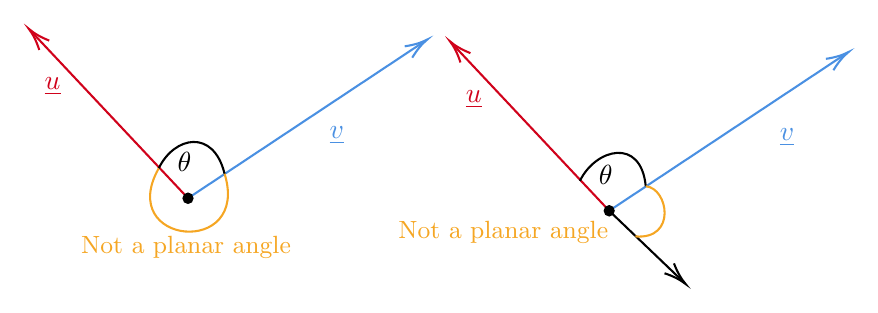
\begin{tikzpicture}[x=0.75pt,y=0.75pt,yscale=-1,xscale=1]
%uncomment if require: \path (0,402); %set diagram left start at 0, and has height of 402

%Straight Lines [id:da4437652617379132] 
\draw [color={rgb, 255:red, 208; green, 2; blue, 27 }  ,draw opacity=1 ]   (184.85,216.98) -- (109.47,136.76) ;
\draw [shift={(108.1,135.3)}, rotate = 46.79] [color={rgb, 255:red, 208; green, 2; blue, 27 }  ,draw opacity=1 ][line width=0.75]    (10.93,-3.29) .. controls (6.95,-1.4) and (3.31,-0.3) .. (0,0) .. controls (3.31,0.3) and (6.95,1.4) .. (10.93,3.29)   ;
%Straight Lines [id:da6919359366246228] 
\draw [color={rgb, 255:red, 74; green, 144; blue, 226 }  ,draw opacity=1 ]   (184.85,216.98) -- (298.51,141.58) ;
\draw [shift={(300.17,140.48)}, rotate = 146.44] [color={rgb, 255:red, 74; green, 144; blue, 226 }  ,draw opacity=1 ][line width=0.75]    (10.93,-3.29) .. controls (6.95,-1.4) and (3.31,-0.3) .. (0,0) .. controls (3.31,0.3) and (6.95,1.4) .. (10.93,3.29)   ;
%Shape: Ellipse [id:dp7599712014506931] 
\draw  [fill={rgb, 255:red, 0; green, 0; blue, 0 }  ,fill opacity=1 ] (182.67,216.98) .. controls (182.67,218.22) and (183.65,219.23) .. (184.85,219.23) .. controls (186.04,219.23) and (187.02,218.22) .. (187.02,216.98) .. controls (187.02,215.75) and (186.04,214.74) .. (184.85,214.74) .. controls (183.65,214.74) and (182.67,215.75) .. (182.67,216.98) -- cycle ;
%Curve Lines [id:da9435159136782311] 
\draw    (170.73,202.58) .. controls (178.25,187.05) and (197.1,183.3) .. (202.47,205.17) ;
%Curve Lines [id:da043732572464616704] 
\draw [color={rgb, 255:red, 245; green, 166; blue, 35 }  ,draw opacity=1 ]   (170.73,202.58) .. controls (149.85,239.67) and (214.99,245.71) .. (202.47,205.17) ;
%Straight Lines [id:da6201503651143601] 
\draw [color={rgb, 255:red, 208; green, 2; blue, 27 }  ,draw opacity=1 ]   (387.77,223.02) -- (312.4,142.8) ;
\draw [shift={(311.03,141.34)}, rotate = 46.79] [color={rgb, 255:red, 208; green, 2; blue, 27 }  ,draw opacity=1 ][line width=0.75]    (10.93,-3.29) .. controls (6.95,-1.4) and (3.31,-0.3) .. (0,0) .. controls (3.31,0.3) and (6.95,1.4) .. (10.93,3.29)   ;
%Straight Lines [id:da44499435743744065] 
\draw [color={rgb, 255:red, 74; green, 144; blue, 226 }  ,draw opacity=1 ]   (387.77,223.02) -- (501.43,147.62) ;
\draw [shift={(503.1,146.51)}, rotate = 146.44] [color={rgb, 255:red, 74; green, 144; blue, 226 }  ,draw opacity=1 ][line width=0.75]    (10.93,-3.29) .. controls (6.95,-1.4) and (3.31,-0.3) .. (0,0) .. controls (3.31,0.3) and (6.95,1.4) .. (10.93,3.29)   ;
%Shape: Ellipse [id:dp13145555074263104] 
\draw  [fill={rgb, 255:red, 0; green, 0; blue, 0 }  ,fill opacity=1 ] (385.6,223.02) .. controls (385.6,224.26) and (386.57,225.26) .. (387.77,225.26) .. controls (388.97,225.26) and (389.94,224.26) .. (389.94,223.02) .. controls (389.94,221.78) and (388.97,220.78) .. (387.77,220.78) .. controls (386.57,220.78) and (385.6,221.78) .. (385.6,223.02) -- cycle ;
%Curve Lines [id:da424029835736604] 
\draw    (373.66,208.62) .. controls (381.18,193.09) and (403.1,187.3) .. (405.39,211.2) ;
%Straight Lines [id:da38053982821885624] 
\draw    (387.77,223.02) -- (423.16,256.92) ;
\draw [shift={(424.6,258.3)}, rotate = 223.77] [color={rgb, 255:red, 0; green, 0; blue, 0 }  ][line width=0.75]    (10.93,-3.29) .. controls (6.95,-1.4) and (3.31,-0.3) .. (0,0) .. controls (3.31,0.3) and (6.95,1.4) .. (10.93,3.29)   ;
%Curve Lines [id:da7344761482411821] 
\draw [color={rgb, 255:red, 245; green, 166; blue, 35 }  ,draw opacity=1 ]   (405.39,211.2) .. controls (416.25,212.07) and (420.43,237.08) .. (400.38,235.36) ;

% Text Node
\draw (114.3,157.54) node [anchor=north west][inner sep=0.75pt]  [color={rgb, 255:red, 208; green, 2; blue, 27 }  ,opacity=1 ] [align=left] {$\displaystyle \underline{u}$};
% Text Node
\draw (251.61,180.86) node [anchor=north west][inner sep=0.75pt]  [color={rgb, 255:red, 74; green, 144; blue, 226 }  ,opacity=1 ] [align=left] {$\displaystyle \underline{v}$};
% Text Node
\draw (178.35,193.32) node [anchor=north west][inner sep=0.75pt]   [align=left] {$\displaystyle \theta $};
% Text Node
\draw (131.86,233.65) node [anchor=north west][inner sep=0.75pt]  [font=\small,color={rgb, 255:red, 245; green, 166; blue, 35 }  ,opacity=1 ] [align=left] {Not a planar angle};
% Text Node
\draw (317.22,163.58) node [anchor=north west][inner sep=0.75pt]  [color={rgb, 255:red, 208; green, 2; blue, 27 }  ,opacity=1 ] [align=left] {$\displaystyle \underline{u}$};
% Text Node
\draw (468.54,181.89) node [anchor=north west][inner sep=0.75pt]  [color={rgb, 255:red, 74; green, 144; blue, 226 }  ,opacity=1 ] [align=left] {$\displaystyle \underline{v}$};
% Text Node
\draw (381.28,199.36) node [anchor=north west][inner sep=0.75pt]   [align=left] {$\displaystyle \theta $};
% Text Node
\draw (284.68,226.75) node [anchor=north west][inner sep=0.75pt]  [font=\small,color={rgb, 255:red, 245; green, 166; blue, 35 }  ,opacity=1 ] [align=left] {Not a planar angle};

\end{tikzpicture}
\end{figure}

Choose the planar angle $\theta$ such that 
$$0 \leq \theta \leq \pi$$.
\end{definition}


\begin{definition}[Scalar Product]

  Let $\vec{v}$ and $\vec{w}$ be two vectors in $\mathbb{E}^3$ and $\theta \in \mathbb{R}$ be the planar angle between them. \\ 
Then, the scalar product of $\vec{v}$ and $\vec{w}$ is defined as:
  \begin{equation}
    \vec{v} \cdot \vec{w} = \mid \vec{v} \mid \mid \vec{w} \mid \cos \theta
  \end{equation}
\end{definition}

\begin{note}
  Two vectors do not lie in the same line, always in the same plane.
  By the convention, the angle $\theta \in [0,\pi] \Rightarrow 0 \leq \theta \leq \pi$.
\end{note}

\subsection{Properties of Scalar Product}
\begin{theorem}[Commutative]
Let $\vec{v}$ and $\vec{w}$ be two vectors in $\mathbb{E}^3$. Then,
  \begin{equation}
    \vec{v} \cdot \vec{w} = \vec{w} \cdot \vec{v}
  \end{equation}
\end{theorem}
\begin{proof}
Since the planar angle $\theta$ is the same for both $\vec{v}$ and $\vec{w}$,
\begin{align*}
  \vec{v} \cdot \vec{w} &= \mid \vec{v} \mid \mid \vec{w} \mid \cos \theta \\
  &= \mid \vec{w} \mid \mid \vec{v} \mid \cos \theta \\
  &= \vec{w} \cdot \vec{v}  
\end{align*}
\end{proof}
\begin{theorem}[Orthogonal Vectors]
 Let $\vec{v}$ and $\vec{w}$ be two vectors in $\mathbb{E}^3$. Then,
  \begin{equation}
    \vec{v} \cdot \vec{w} = 0 \iff \vec{v} \perp \vec{w}
  \end{equation} 
\end{theorem}
\begin{proof}
When $\vec{v} \perp \vec{w}$, the planar angle $\theta = \frac{\pi}{2}$. 
Therefore, 
\begin{align*}
  \vec{v} \cdot \vec{w} &= \mid \vec{v} \mid \mid \vec{w} \mid \cos \theta \\
  &= \mid \vec{v} \mid \mid \vec{w} \mid \cos \frac{\pi}{2} \\
  &= \mid \vec{v} \mid \mid \vec{w} \mid \cdot 0 \\
  &= 0
\end{align*}
  i.e. $\vec{v}$ and $\vec{w}$ are orthogonal.
\end{proof}

\begin{theorem}[Distributivity over scalar multiplication]
  Let $\vec{v}, \vec{w} \in \mathbb{E}^3$ and $\lambda \in \mathbb{R}$. Then,
  \begin{equation}
    \lambda(\vec{v} \cdot \vec{w}) = (\lambda \vec{v}) \cdot \vec{w} = \vec{v} \cdot (\lambda \vec{w})
  \end{equation}
\end{theorem}

\begin{theorem}[Distributivity over Addition]
  Let $\vec{u}, \vec{v}, \vec{w} \in \mathbb{E}^3$. Then,
  \begin{equation}
    \vec{u} \cdot (\vec{v} + \vec{w}) = \vec{u} \cdot \vec{v} + \vec{u} \cdot \vec{w}
  \end{equation}
\end{theorem}

\begin{note}
  Properties of scalar product for standard basis vectors:
  \begin{align*}
    \hat{i} \cdot \hat{i} &= 1 \\
    \hat{j} \cdot \hat{j} &= 1 \\
    \hat{k} \cdot \hat{k} &= 1 \\
    \hat{i} \cdot \hat{j} &= 0 \\
    \hat{i} \cdot \hat{k} &= 0 \\
    \hat{j} \cdot \hat{k} &= 0 \\
  \end{align*}
\end{note}

\subsection{Scalar Product in terms of Components}
\vspace{5px}
\begin{theorem}
  Let $\vec{v} = (v_1, v_2, v_3)$ and $\vec{w} = (w_1, w_2, w_3)$ be two vectors in $\mathbb{E}^3$. Then,
  \begin{equation}
    \vec{v} \cdot \vec{w} = \sum_{i=1}^{3}v_{i}w_{i} = v_1w_1 + v_2w_2 + v_3w_3
  \end{equation}
\end{theorem}
\begin{proof}
  Let $\vec{v}, \vec{w} \in \mathbb{E}^{3}$. Then, 
  \begin{flalign*}
    \vec{v} \cdot \vec{w} &= (v_1 \hat{i} + v_2 \hat{j} + v_3 \hat{k}) \cdot (w_1 \hat{i} + w_2 \hat{j} + w_3 \hat{k}) &\\ \\ 
      &= v_{1} \cdot (w_{1} \hat{i} + w_{2}\hat{j} + w_3 \hat{k}) + v_{2} \cdot (w_{1} \hat{i} + w_{2}\hat{j} + w_3 \hat{k}) + v_{3} \cdot (w_{1} \hat{i} + w_{2}\hat{j} + w_3 \hat{k})   &\\ \\
      &= v_{1}w_{1} \hat{i} \cdot \hat{i} + \cancel{v_{1}w_{2} \hat{i} \cdot \hat{j}} + \cancel{v_{1}w_{3} \hat{i} \cdot \hat{k}}  + \cancel{v_{2}w_{1} \hat{j} \cdot \hat{i}} + v_{2}w_{2} \hat{j} \cdot \hat{j} + \cancel{v_{2}w_{3} \hat{j} \cdot \hat{k}} \\  &+ \cancel{v_{3}w_{1} \hat{k} \cdot \hat{i}} + \cancel{v_{3}w_{2} \hat{k} \cdot \hat{j}} + v_{3}w_{3} \hat{k} \cdot \hat{k} &\\ \\
      &= v_{1}w_{1} + v_{2}w_{2} + v_{3}w_{3} &\\ \\ 
      &= \sum_{i=1}^{3}v_{i}w_{i} = v_1w_1 + v_2w_2 + v_3w_3
  \end{flalign*}
\end{proof}

\subsection{Using Scalar Product to find the length of a vector}
We can also use scalar product to find the length of a vector.
\begin{theorem}
  Let $\vec{v} \in \mathbb{E}^3$. Then,
  \begin{equation}
    \mid \vec{v} \mid = \sqrt{\vec{v} \cdot \vec{v}}
  \end{equation}
\end{theorem}
\begin{proof}
Let $\vec{v} \in \mathbb{E}^3$. Then,
  \begin{flalign*}
    \mid \vec{v} \mid &= \sqrt{v_1^{2} + v_2^{2} + v_3^{2}} \\ \\ 
    &= \sqrt{v_1v_1 + v_2v_2 + v_3v_3}  \\ \\
    &= \sqrt{\vec{v} \cdot \vec{v}}  
  \end{flalign*}
\end{proof}

\subsection{Using Scalar Product to find the angle between two vectors}

\begin{theorem}
  Let $\vec{v}, \vec{w} \in \mathbb{E}^3$. Then, the planar angle $\theta$ between $\vec{v}$ and $\vec{w}$ is given by:
  \begin{equation}
    \theta = \cos^{-1} \left( \frac{\vec{v} \cdot \vec{w}}{\mid \vec{v} \mid \mid \vec{w} \mid} \right)
  \end{equation}
\end{theorem}
\begin{proof}
  Let $\vec{v}, \vec{w} \in \mathbb{E}^3$. Then,
  \begin{flalign*}
    \vec{v} \cdot \vec{w} &= \mid \vec{v} \mid \mid \vec{w} \mid \cos \theta  \\ \\
    &= v_1w_1 + v_2w_2 + v_3w_3 \\ \\
    \Rightarrow \cos \theta &= \frac{v_1w_1 + v_2w_2 + v_3w_3}{\mid \vec{v} \mid \mid \vec{w} \mid} \\ \\
    \Rightarrow \theta &= \cos^{-1} \left( \frac{\vec{v} \cdot \vec{w}}{\mid \vec{v} \mid \mid \vec{w} \mid} \right)
  \end{flalign*}
\end{proof}

\begin{note}
  Some basic properties of scalar product:
  \begin{enumerate}
    \item If $\vec{v} \cdot \vec{w} = 0$, then $\theta = \frac{\pi}{2}$.
    \item If $\vec{v} \cdot \vec{w} > 0$, then $\theta \in [0, \frac{\pi}{2})$.
    \item If $\vec{v} \cdot \vec{w} < 0$, then $\theta \in (\frac{\pi}{2}, \pi]$.
  \end{enumerate}
\end{note}
